\documentclass[a4paper,12pt]{article}

\usepackage[T2A]{fontenc}			
\usepackage[utf8]{inputenc}			
\usepackage[english,russian]{babel}	

\usepackage[
bookmarks=true, colorlinks=true, unicode=true,
urlcolor=black,linkcolor=black, anchorcolor=black,
citecolor=black, menucolor=black, filecolor=black,
]{hyperref}

\usepackage{color}
\usepackage{caption}
\DeclareCaptionFont{white}{\color{black}}
\DeclareCaptionFormat{listing}{\colorbox{white}{\parbox{\textwidth}{#1#2#3}}}
\captionsetup[lstlisting]{format=listing,labelfont=white,textfont=white}

\usepackage{amsmath,amsfonts,amssymb,amsthm,mathtools} 
\usepackage{wasysym}

\usepackage{graphicx}
%\usepackage[cache=false]{minted}
\usepackage{cmap}
\usepackage{indentfirst}

\usepackage{listings} 
\usepackage{fancyvrb}

\usepackage{geometry}
\geometry{left=2cm}
\geometry{right=1.5cm}
\geometry{top=1cm}
\geometry{bottom=2cm}

\setlength{\parindent}{5ex}
\setlength{\parskip}{0.5em}

\usepackage{pgfplots}
\usetikzlibrary{datavisualization}
\usetikzlibrary{datavisualization.formats.functions}

\begin{document}
	
	\begin{figure}[h!]
		\begin{center}
			{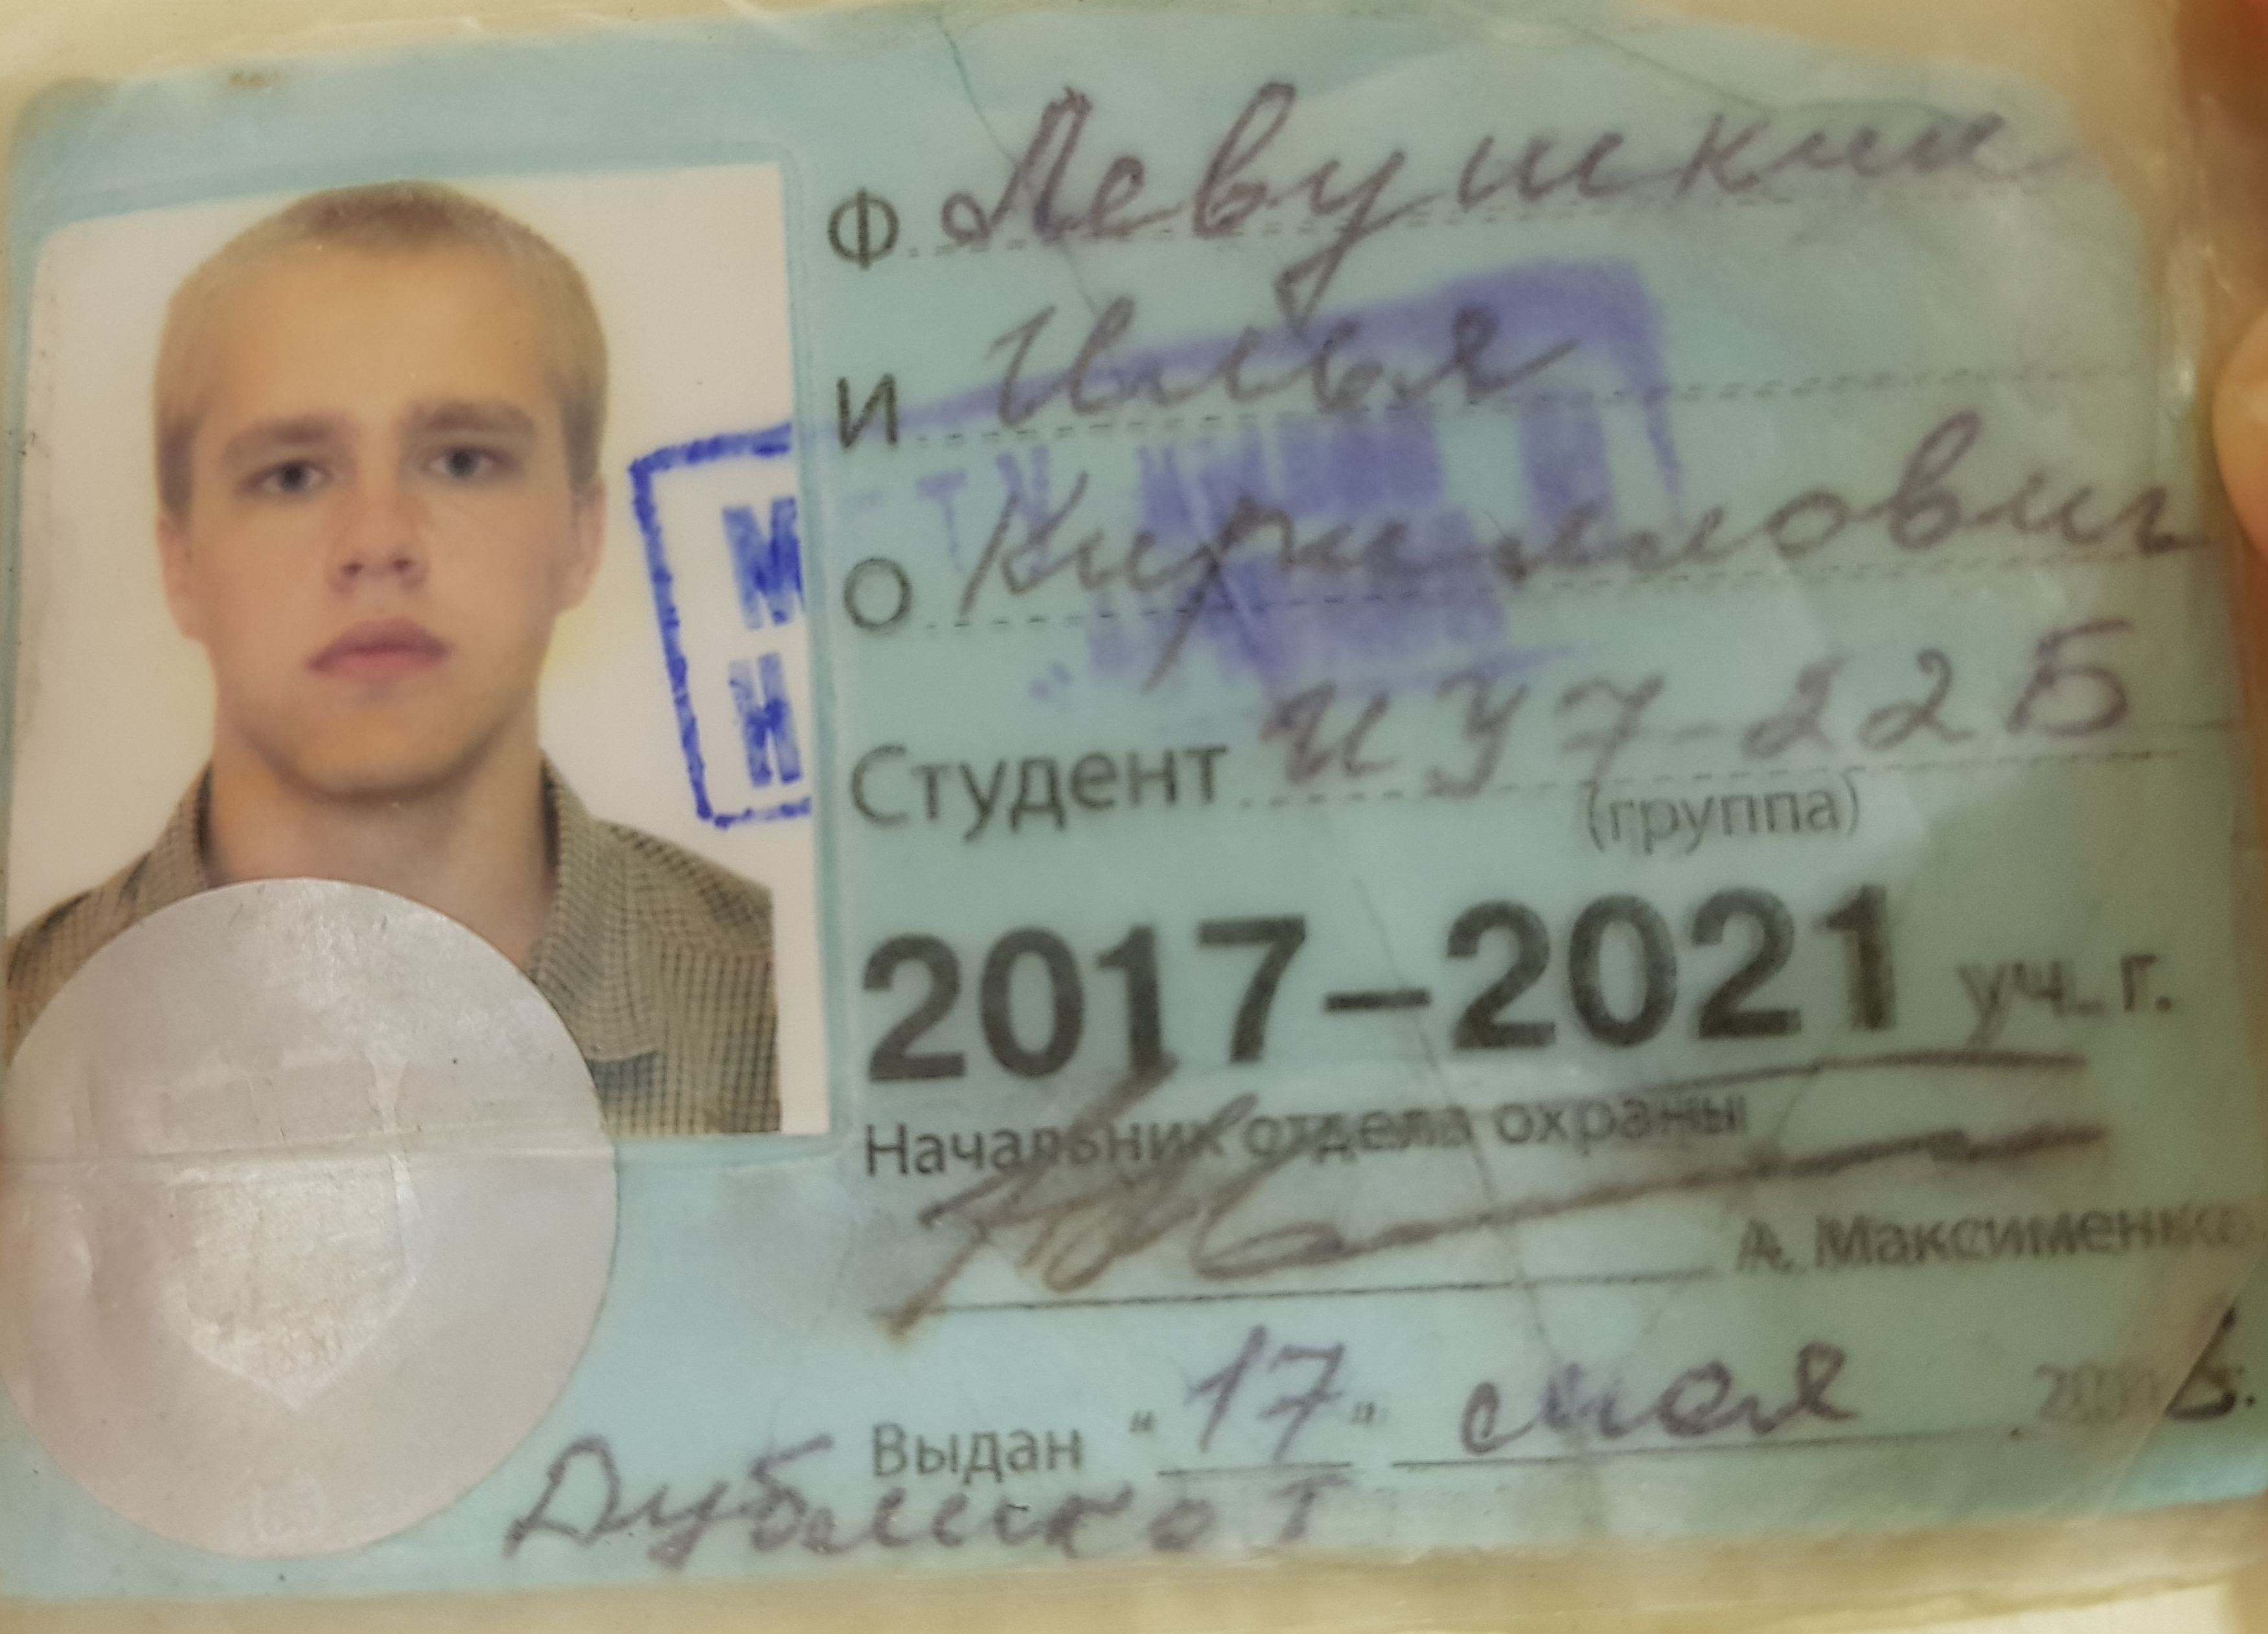
\includegraphics[scale = 0.15]{photo_ilya.jpg}}
			\label{ilya}
		\end{center}
	\end{figure}

	\begin{figure}[h!]
		\begin{center}
			{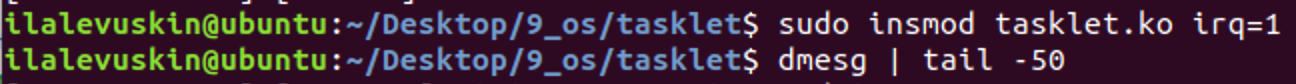
\includegraphics[scale = 0.9,  angle = 180]{1.jpg}}
			\label{1}
		\end{center}
	\end{figure}
	
	\newpage
	
	\begin{figure}[h!]
		\begin{center}
			{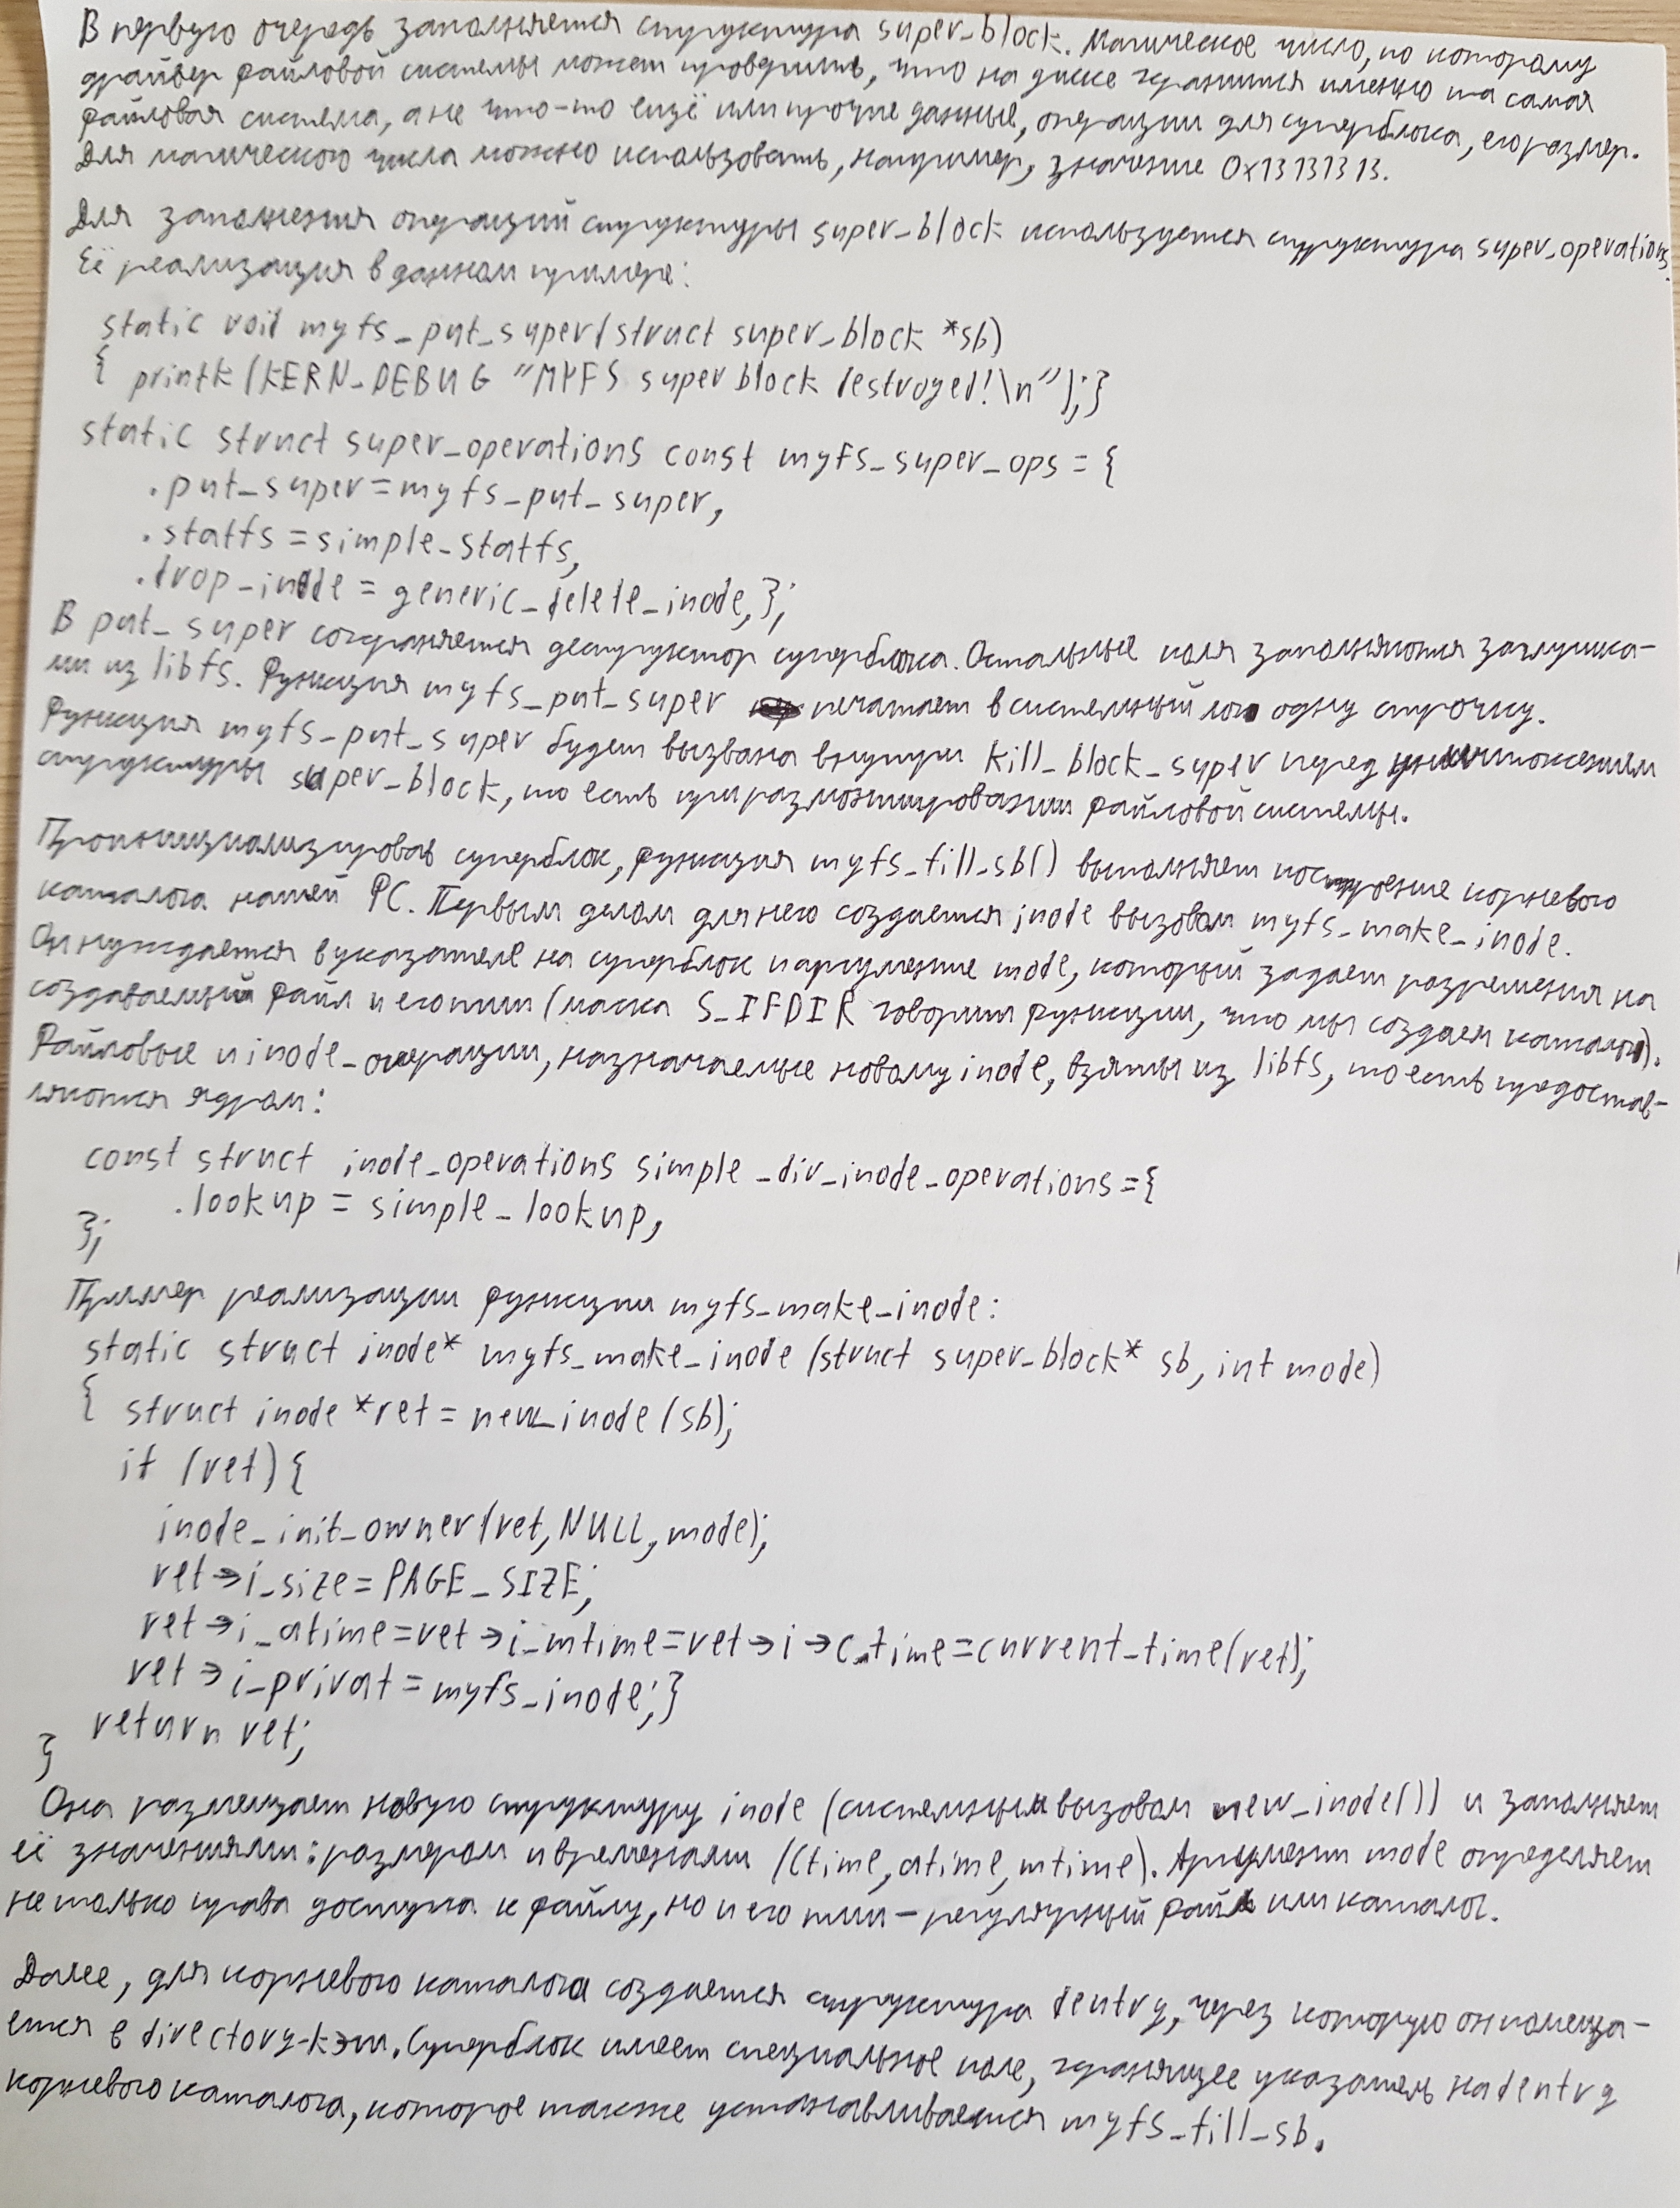
\includegraphics[scale = 0.9,  angle = 180]{2.jpg}}
			\label{2}
		\end{center}
	\end{figure}
	
	\newpage
	
	\begin{figure}[h!]
		\begin{center}
			{
\includegraphics[scale = 0.9,  angle = 180]{3.jpg}}
			\label{3}
		\end{center}
	\end{figure}

	\begin{figure}[h!]
		\begin{center}
			{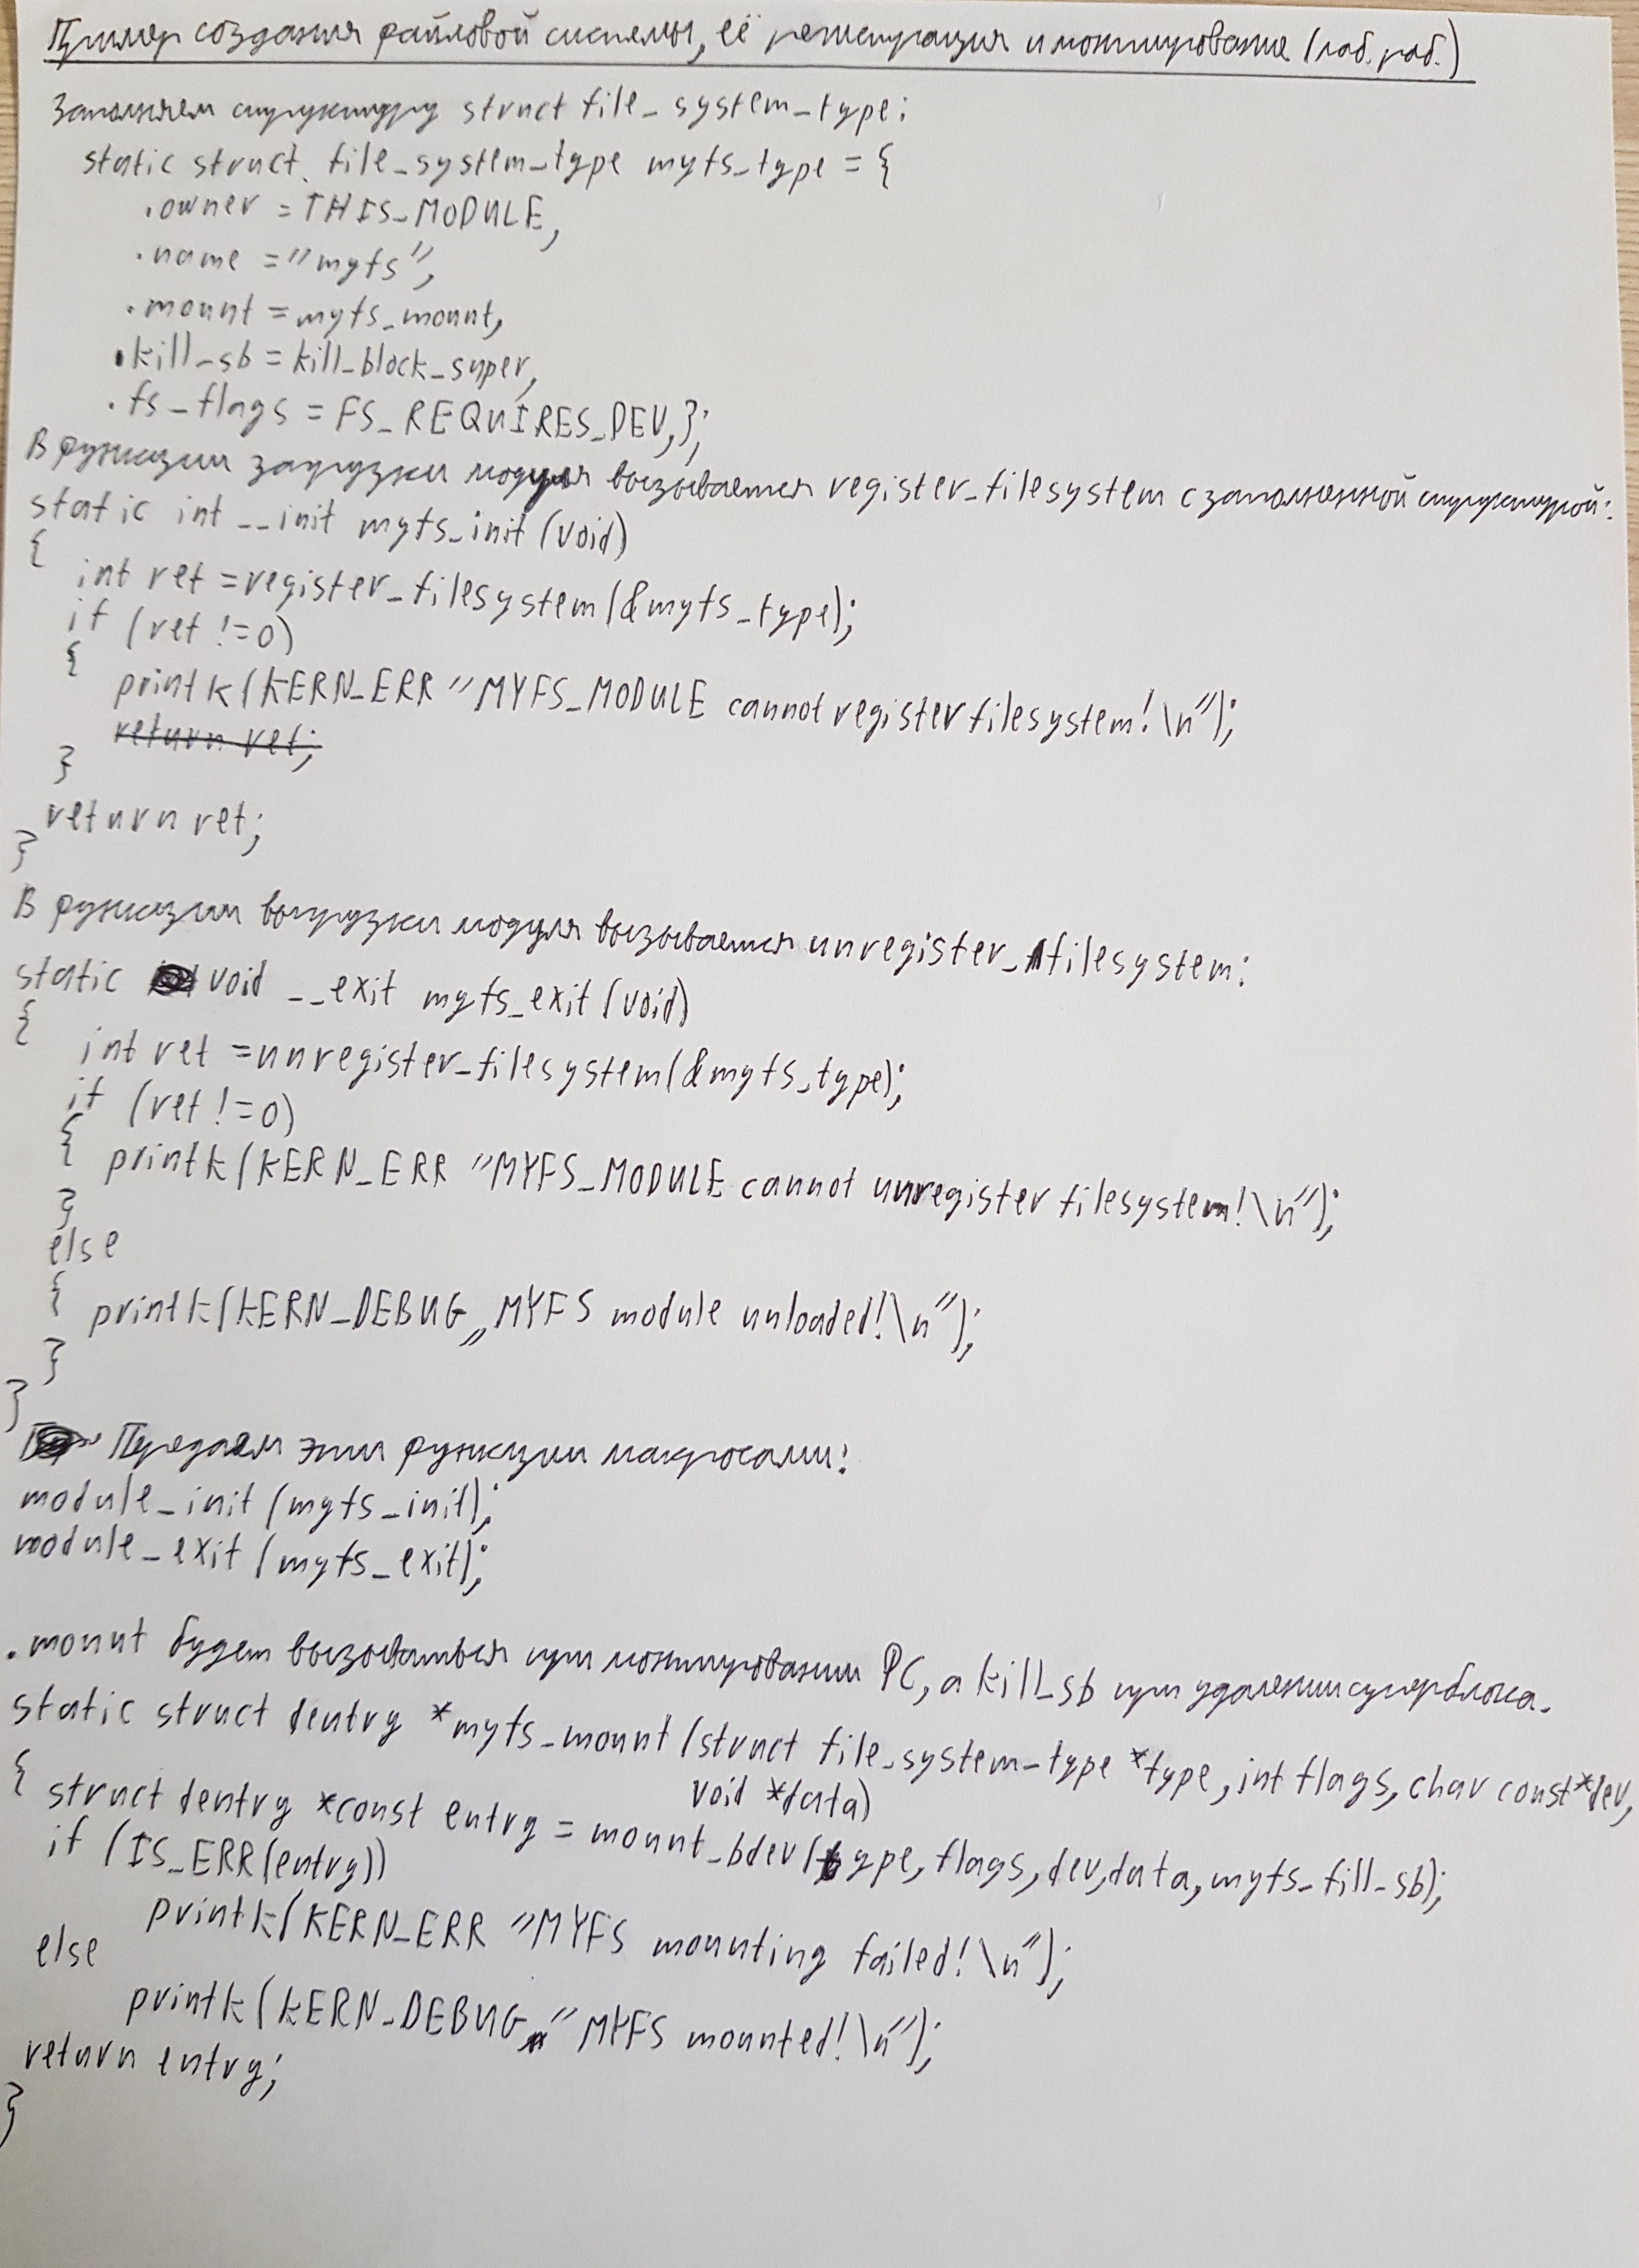
\includegraphics[scale = 0.9,  angle = 180]{4.jpg}}
			\label{4}
		\end{center}
	\end{figure}


	
\end{document}